% Observed rounded source glyph, cote 119, site 42, PDF page 43.
% Its conventional alphabet assignment remains uncertain; use with \unsure.
% The contour is a vector traced from the reviewed scan detail, not a font alias.
\makeatletter
\newcommand{\sourceglyph}[1]{\mathord{\mathpalette{\EditionSourceGlyph{#1}}{}}}
\newcommand{\EditionSourceGlyph}[3]{%
  \begingroup
  \setbox0=\hbox{$#2 A$}%
  \resizebox{!}{\ht0}{\csname EditionGlyph@#1\endcsname}%
  \endgroup}
\expandafter\newcommand\csname EditionGlyph@119A\endcsname{%
  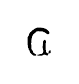
\begin{tikzpicture}[x=1pt,y=1pt,baseline=0pt]
  \path[fill,even odd rule]
(3.450,10.100) -- (4.950,10.100) -- (5.050,10.000) -- (5.550,10.000) -- (5.650,9.900) -- (5.950,9.900) -- (6.050,9.800) -- (6.250,9.800) -- (6.650,9.600) -- (6.950,9.300) -- (7.050,9.300) -- (7.600,8.750) -- (7.800,8.350) -- (7.800,8.050) -- (7.550,7.800) -- (7.050,7.800) -- (6.250,8.400) -- (6.050,8.500) -- (5.850,8.500) -- (5.350,8.800) -- (3.950,8.800) -- (3.850,8.900) -- (3.650,8.900) -- (3.550,8.800) -- (3.350,8.800) -- (3.150,8.700) -- (2.250,7.900) -- (2.100,7.850) -- (2.100,7.750) -- (1.900,7.550) -- (1.500,6.750) -- (1.500,6.450) -- (1.400,6.350) -- (1.400,5.850) -- (1.300,5.750) -- (1.300,4.650) -- (1.200,4.550) -- (1.200,4.050) -- (1.300,3.950) -- (1.300,2.450) -- (1.400,2.350) -- (1.400,2.150) -- (1.700,1.850) -- (1.900,1.450) -- (1.900,1.250) -- (2.000,1.050) -- (2.150,1.000) -- (2.550,0.600) -- (2.850,0.500) -- (3.100,0.250) -- (3.100,0.150) -- (2.850,0.000) -- (2.250,0.000) -- (2.050,0.100) -- (1.750,0.400) -- (1.650,0.400) -- (0.900,1.150) -- (0.900,1.350) -- (0.700,1.650) -- (0.700,1.850) -- (0.500,2.050) -- (0.300,2.450) -- (0.300,2.750) -- (0.200,2.850) -- (0.200,3.150) -- (0.100,3.250) -- (0.100,3.850) -- (0.000,3.950) -- (0.000,6.650) -- (0.300,7.050) -- (0.400,7.250) -- (0.400,7.450) -- (0.500,7.550) -- (0.500,7.750) -- (0.700,7.950) -- (0.800,8.250) -- (1.950,9.300) -- (2.050,9.300) -- (2.550,9.700) -- (3.150,10.000) -- (3.350,10.000) -- (3.450,10.100) -- cycle
(6.050,5.700) -- (6.250,5.700) -- (6.500,5.450) -- (6.500,5.250) -- (6.600,5.150) -- (6.600,4.650) -- (6.500,4.550) -- (6.500,2.850) -- (6.400,2.750) -- (6.500,2.550) -- (6.500,2.050) -- (6.600,1.950) -- (6.600,1.250) -- (6.950,0.900) -- (7.500,0.750) -- (7.400,0.550) -- (7.400,0.350) -- (7.250,0.100) -- (6.850,0.100) -- (6.250,0.400) -- (5.850,0.400) -- (5.150,0.000) -- (4.750,0.000) -- (4.650,0.100) -- (4.550,0.000) -- (3.650,0.000) -- (3.500,0.150) -- (3.550,0.300) -- (3.750,0.400) -- (4.250,0.400) -- (4.350,0.500) -- (4.850,0.500) -- (4.950,0.600) -- (5.150,0.600) -- (5.500,0.950) -- (5.600,1.150) -- (5.600,1.350) -- (5.700,1.450) -- (5.700,1.950) -- (5.600,2.050) -- (5.600,2.350) -- (5.500,2.450) -- (5.500,2.750) -- (5.400,2.850) -- (5.400,3.350) -- (5.500,3.450) -- (5.500,4.050) -- (5.600,4.150) -- (5.600,5.050) -- (5.800,5.450) -- (6.050,5.700) -- cycle
(7.950,1.900) -- (8.300,1.850) -- (8.300,1.050) -- (8.150,0.900) -- (7.950,0.900) -- (7.850,0.800) -- (7.550,0.800) -- (7.500,0.950) -- (7.600,1.050) -- (7.600,1.450) -- (7.950,1.900) -- cycle;
  \end{tikzpicture}}
\makeatother
